\documentclass{article}
\usepackage[T1]{fontenc}
\usepackage[polish]{babel}
\usepackage[utf8]{inputenc}
\usepackage{graphicx} % Required for inserting images
\usepackage{amsmath}
\usepackage{listings} % code highlighting
\usepackage{xcolor}
\usepackage{float}

\definecolor{codegreen}{rgb}{0,0.6,0}
\definecolor{codegray}{rgb}{0.5,0.5,0.5}
\definecolor{codepurple}{rgb}{0.58,0,0.82}
\definecolor{backcolour}{rgb}{0.95,0.95,0.92}

\lstdefinestyle{mystyle}{
    backgroundcolor=\color{backcolour},
    commentstyle=\color{codegreen},
    keywordstyle=\color{magenta},
    numberstyle=\tiny\color{codegray},
    stringstyle=\color{codepurple},
    basicstyle=\ttfamily\footnotesize,
    breakatwhitespace=false,
    breaklines=true,
    captionpos=b,
    keepspaces=true,
    numbers=left,
    numbersep=5pt,
    showspaces=false,
    showstringspaces=false,
    showtabs=false, 
    tabsize=2
}

\lstset{style=mystyle}
\lstset{ % polish letters in code blocks
  literate={ą}{{\k a}}1
  		     {Ą}{{\k A}}1
           {ż}{{\. z}}1
           {Ż}{{\. Z}}1
           {ź}{{\' z}}1
           {Ź}{{\' Z}}1
           {ć}{{\' c}}1
           {Ć}{{\' C}}1
           {ę}{{\k e}}1
           {Ę}{{\k E}}1
           {ó}{{\' o}}1
           {Ó}{{\' O}}1
           {ń}{{\' n}}1
           {Ń}{{\' N}}1
           {ś}{{\' s}}1
           {Ś}{{\' S}}1
           {ł}{{\l}}1
           {Ł}{{\L}}1
}

\title{MOwNiT - Laboratorium 11:\\
Całkowanie Monte Carlo}
\author{Wojciech Dąbek}
\date{4 czerwca 2024}

\begin{document}

\maketitle

\section{Treści zadań}

Tematem zadania będzie obliczenie metodą Monte Carlo całki funkcji:
\begin{enumerate}
    \item \(x^2 + x + 1\)
    \item \(\sqrt{1 - x^2}\)
    \item \(\frac{1}{\sqrt{x}}\)
\end{enumerate}
w przedziale \((0,\ 1)\).

\vspace{5mm}
\noindent
Proszę dla tych funkcji:
\begin{enumerate}
    \item Napisać funkcję liczącą całkę metodą "hit-and-miss".\\
    Czy będzie ona dobrze działać dla funkcji \(\frac{1}{\sqrt{x}}\)?
    \item Policzyć całkę przy użyciu napisanej funkcji.\\
    Jak zmienia się błąd wraz ze wzrostem liczby prób?
    \item Policzyć wartość całki korzystając ze wzoru prostokątów dla dokładności 1e-3, 1e-4, 1e-5 i 1e-6. Porównać czas obliczenia całki metodą Monte Carlo i przy pomocy wzoru prostokątów dla tej samej dokładności.\\
    Narysować wykres. Zinterpretować wyniki.
\end{enumerate}

\newpage

\section{Rozwiązania}

\subsection{Zadanie 1}

\noindent
Zadaną funkcję (wraz z pomocniczą określającą wysokość obszaru) napisałem w języku Python:
\begin{lstlisting}[language=Python]
from random import uniform  # liczby quasi-losowe
                            # (rozkład jednostajny)

def estimate_maximum(f, a, b):
    if a == 0:
        a = .0001
    cur = f(a)
    d = min((b - a) / 100, .5)
    x = a
    while x < b:
        cur = max(cur, f(x))
        x += d
    return cur * 1.1


def monte_carlo(f, a, b, n):
    counter = 0
    h = estimate_maximum(f, a, b)
    for _ in range(n):
        x = uniform(a, b)
        y = uniform(0, h)
        if y <= f(x):
            counter += 1
    return (b - a) * h * counter / n
\end{lstlisting}
Ponieważ \(\lim_{x \to 0^+} \frac{1}{\sqrt{x}} = +\infty\), dla przedziału \((0,\ 1)\) funkcja \verb|estimate_maximum| zwróci bardzo dużą wysokość rozważanego obszaru, którego pole pod wykresem początkowo bardzo szybko malejącej funkcji będzie bardzo małą częścią. Z tego powodu przy małej ilości wybranych punktów otrzymana ostatecznie przybliżona wartość funkcji może być względem dokładnej bardzo zaniżona (czy wręcz zerowa).

\vspace{5mm}
\noindent
\textbf{Wniosek:} Metoda ta nie sprawdzi się dobrze do całkowania funkcji, które przyjmują na niewielkich fragmentach rozważanego przedziału wartości mocno odbiegające rzędem wielkości od wartości na większości tego przedziału.

\newpage

\subsection{Zadanie 2}

Aby określić błędy, potrzebujemy najpierw obliczyć analitycznie wartości całek:
\begin{gather*}
    \int_0^1 (x^2 + x + 1)\ dx = \frac{11}{6}\\
    \int_0^1 \sqrt{1 - x^2}\ dx = \frac{\pi}{4}\\
    \int_0^1 \frac{dx}{\sqrt{x}} = 2
\end{gather*}

\noindent
Wartości całek dla zadanych funkcji wraz z błędami bezwzględymi dla liczby prób od 10 do \(10^6\) obliczam następującym kodem korzystającym z funkcji z zadania 1:
\begin{lstlisting}[language=Python]
from math import sqrt, pi, fabs

x_0, x_n = 0, 1
funs = [
    (lambda x: x * x + x + 1, 11/6, 'x^2 + x + 1'),
    (lambda x: sqrt(1 - x * x), pi/4, 'sqrt(1 - x^2)'),
    (lambda x: 1 / sqrt(x), 2, '1 / sqrt(x)')
]

for i, (fun, exact, rep) in enumerate(funs):
    print(f'f(x) = {rep}')
    for k in range(1, 7):
        N = 10**k
        result = monte_carlo(fun, x_0, x_n, N)
        print(f'for N = 10^{k}: {result:.4f}', end='\t')
        print(f'error = {fabs(exact - result):.4f}')
    print()
\end{lstlisting}
Program ten wypisuje:

\begin{verbatim}
f(x) = x^2 + x + 1
for N = 10^1: 1.3200    error = 0.5133
for N = 10^2: 1.5840    error = 0.2493
for N = 10^3: 1.8579    error = 0.0246
for N = 10^4: 1.8355    error = 0.0021
for N = 10^5: 1.8360    error = 0.0026
for N = 10^6: 1.8336    error = 0.0003

f(x) = sqrt(1 - x^2)
for N = 10^1: 0.5500    error = 0.2354
for N = 10^2: 0.9460    error = 0.1606
for N = 10^3: 0.7898    error = 0.0044
for N = 10^4: 0.7905    error = 0.0051
for N = 10^5: 0.7873    error = 0.0019
for N = 10^6: 0.7853    error = 0.0001

f(x) = 1 / sqrt(x)
for N = 10^1: 0.0000    error = 2.0000
for N = 10^2: 0.0000    error = 2.0000
for N = 10^3: 2.2000    error = 0.2000
for N = 10^4: 2.0460    error = 0.0460
for N = 10^5: 2.0152    error = 0.0152
for N = 10^6: 1.9861    error = 0.0139
\end{verbatim}
Możemy zaobserwować konsekwentny spadek wartości błędu wraz ze wzrostem liczby prób. Potwierdzony jest też wniosek z zadania 1.

\subsection{Zadanie 3}

Obliczenia oraz rysowanie wykresów wykonałem następującym programem wykorzystującym funkcje z zadania 1:

\begin{lstlisting}[language=Python]
from time import perf_counter
import matplotlib.pyplot as plt


def rect_integrate(f, a, b, h):
    if a == 0:
        a = .0001
    sum = 0
    x = a
    while x < b:
        sum += f(x)
        x += h
    return sum * h


x_0, x_n = 0, 1
funs = [
    (lambda x: x * x + x + 1, 11/6, 'x^2 + x + 1'),
    (lambda x: sqrt(1 - x * x), pi/4, 'sqrt(1 - x^2)'),
    (lambda x: 1 / sqrt(x), 2, '1 / sqrt(x)')
]

for i, (fun, _, rep) in enumerate(funs):
    print(f'f(x) = {rep}')
    mc_times, rect_times = [], []
    for k in range(3, 7):
        N = 10**k
        time = perf_counter()
        mc_result = monte_carlo(fun, x_0, x_n, N)
        time = perf_counter() - time
        print(f'for N = 10^{k}:  {mc_result:.4f}', end='\t')
        print(f'time = {time:.5f} s')
        mc_times.append(time)
        time = perf_counter()
        rect_result = rect_integrate(fun, x_0, x_n, 1/N)
        time = perf_counter() - time
        print(f'for h = 10^-{k}: {rect_result:.4f}', end='\t')
        print(f'time = {time:.5f} s')
        rect_times.append(time)
    print()
    plt.plot(range(3, 7), mc_times, label='monte carlo')
    plt.plot(range(3, 7), rect_times, label='rectangle rule')
    plt.legend(loc='upper left')
    plt.title('Comparison of method times')
    plt.xlabel('precision [10^k]')
    plt.ylabel('time [s]')
    plt.show()
\end{lstlisting}
Program wypisuje:
\begin{verbatim}
f(x) = x^2 + x + 1
for N = 10^3:  1.8513	time = 0.00047 s
for h = 10^-3: 1.8325	time = 0.00014 s
for N = 10^4:  1.8434	time = 0.00447 s
for h = 10^-4: 1.8334	time = 0.00132 s
for N = 10^5:  1.8285	time = 0.04407 s
for h = 10^-5: 1.8333	time = 0.01345 s
for N = 10^6:  1.8354	time = 0.44108 s
for h = 10^-6: 1.8332	time = 0.13260 s

f(x) = sqrt(1 - x^2)
for N = 10^3:  0.7777	time = 0.00055 s
for h = 10^-3: 0.7858	time = 0.00020 s
for N = 10^4:  0.7878	time = 0.00538 s
for h = 10^-4: 0.7853	time = 0.00198 s
for N = 10^5:  0.7811	time = 0.05297 s
for h = 10^-5: 0.7853	time = 0.01987 s
for N = 10^6:  0.7855	time = 0.58076 s
for h = 10^-6: 0.7853	time = 0.19799 s

f(x) = 1 / sqrt(x)
for N = 10^3:  1.7600	time = 0.00052 s
for h = 10^-3: 2.0494	time = 0.00018 s
for N = 10^4:  1.8370	time = 0.00510 s
for h = 10^-4: 1.9854	time = 0.00188 s
for N = 10^5:  1.9987	time = 0.05079 s
for h = 10^-5: 1.9805	time = 0.01951 s
for N = 10^6:  1.9950	time = 0.50160 s
for h = 10^-6: 1.9800	time = 0.18567 s
\end{verbatim}

\newpage

\noindent
Oraz rysuje następujące wykresy:

\begin{figure}[H]
    \centering
    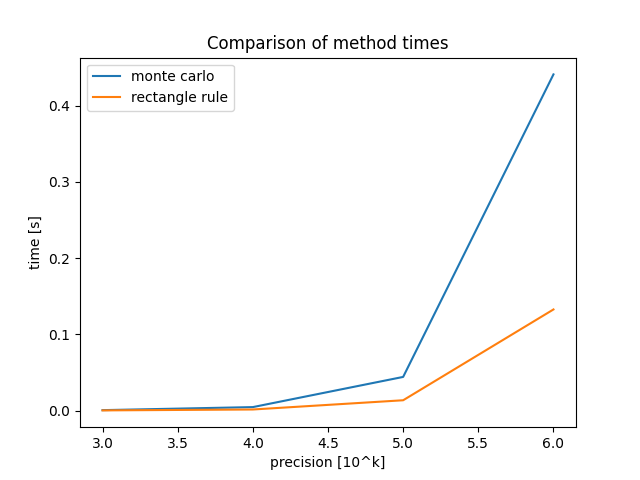
\includegraphics[width=0.85\linewidth]{plots/plot1.png}
    \caption{Wykres czasu obliczeń dla funkcji \(x^2 + x + 1\)}
    \label{fig:plot1}
\end{figure}

\begin{figure}[H]
    \centering
    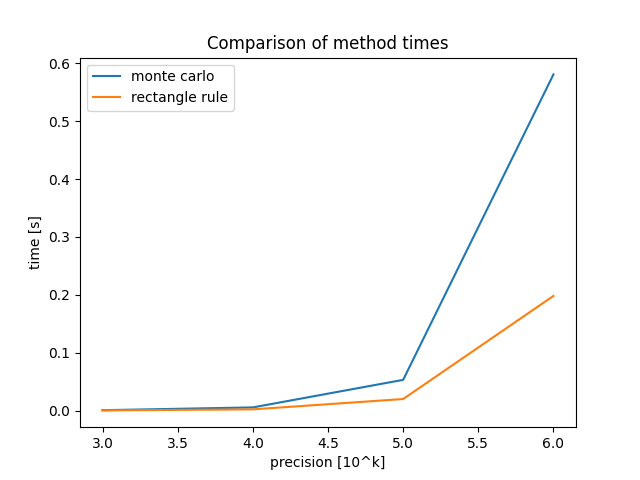
\includegraphics[width=0.85\linewidth]{plots/plot2.png}
    \caption{Wykres czasu obliczeń dla funkcji \(\sqrt{1 - x^2}\)}
    \label{fig:plot2}
\end{figure}

\begin{figure}[H]
    \centering
    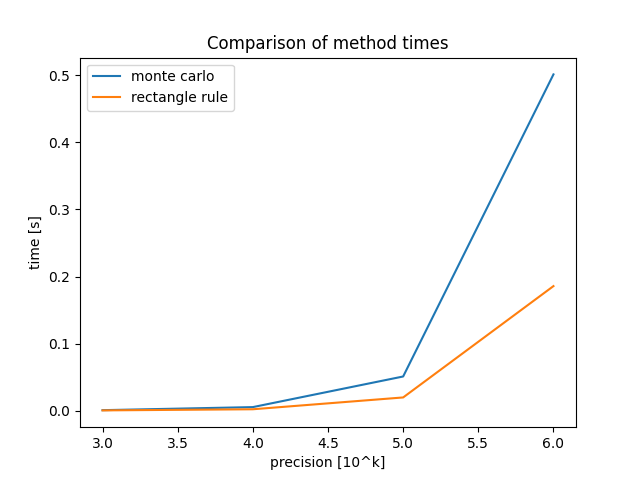
\includegraphics[width=0.85\linewidth]{plots/plot3.png}
    \caption{Wykres czasu obliczeń dla funkcji \(\frac{1}{\sqrt{x}}\)}
    \label{fig:plot3}
\end{figure}

\noindent
\textbf{Wniosek:} Czas obliczeń w obu przypadkach rośnie w podobny sposób, ale szybciej w przypadku metody Monte Carlo niż prostokątów. Zależność tak jest prawdziwa w ten sam sposób dla wszystkich badanych funkcji.

\section{Bibliografia}
Materiały ze strony

\end{document}
